\section{Introduction}
\label{sec:intro}

In recent years, Transformers \cite{vaswani2017attention} have emerged as the universal architecture for modern foundation models across many modalities, from text \cite{raffel2023exploring, chowdhery2022palm, radford2018improving,brown2020language} to audio \cite{li2018close, Wang_2017}, and images \cite{dosovitskiy2021image, Carion_2020}. Among these, Vision Transformers (ViTs) \cite{dosovitskiy2021image}
trained at scale not only achieve state-of-the-art under multiple benchmarks but also exhibit intriguing behaviors and capabilities across various tasks \cite{caron2021emerging,he2022masked,radford2021learning,oquab2023dinov2}.




Despite these significant strides made by ViTs, our work reveals a crucial yet often overlooked challenge: the presence of persistent noise artifacts in ViT outputs, observable across various training algorithms \cite{dosovitskiy2021image, oquab2023dinov2,touvron2022deit,radford2021learning,fang2023eva,caron2021emerging} (illustrated in \cref{fig:teaser} left). These artifacts not only compromise visual clarity but also hinder feature interpretability and disrupt semantic coherence.
For example, \cref{fig:clustering} demonstrates that applying clustering algorithms directly on the raw ViT output results in noisy clusters, and the patch feature similarity is less reliable. 
Additionally, these artifacts are frequently concealed by \textit{seemingly} impressive performance on downstream tasks, thus evading thorough examination or detection by the research community.
Addressing these artifacts can unleash the potential of pre-trained ViTs and lead to substantial performance improvements (\cref{fig:teaser} right). Therefore, our work aims to answer a crucial research question: \textit{Is it feasible to effectively denoise these artifacts in pre-trained ViTs, ideally without model retraining?}

%##################################################################################################
\begin{figure}[t!]
    \centering
    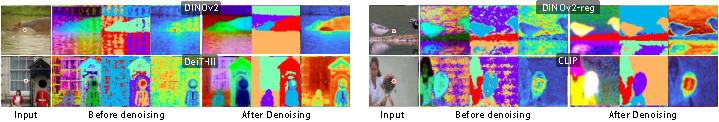
\includegraphics[width=\linewidth]{figures/fig2_coherence.pdf}
    \caption{\textbf{Artifacts hurt semantic coherence.} For each triplet, we show a feature map, a K-Means cluster map, and a similarity map of the central patch (red dotted) with other patches in the image. Observe how artifacts negatively impact clustering accuracy and similarity correspondences, and how our denoising mitigates these issues.}
    \label{fig:clustering}
\end{figure}
%##################################################################################################

To answer this, we first investigate the origins of these artifacts. We hypothesize that positional embeddings, a fundamental component of ViT architecture, play a pivotal role in the emergence of these artifacts. Our initial analysis supports this hypothesis: \textit{First}, when a zero tensor is fed into a pre-trained DINOv2 model \cite{oquab2023dinov2}, the resulting output is predominantly characterized by similar noise patterns (\cref{fig:vit_arch}-(a, 2)). \textit{Second}, we observe the absence of such artifacts in the outputs of a DINOv2 model trained without positional embeddings,  which contrasts sharply with the standard model outputs (\cref{fig:vit_arch}-(a, 1) v.s. (a, 3)).
\textit{Third}, take a video with continuous frames as an example (\cref{fig:vit_arch}-(c)). Despite the significant differences in the context of various input frames, the artifacts maintain a generally consistent relative position in the images (\cref{fig:vit_arch}-(c), middle row).



With these insights, we present a two-stage denoising approach, \ourslong (\ours), to suppress artifacts in pre-trained ViTs. In the first stage, we obtain clean features from contaminated ones by enforcing cross-view feature consistency and artifact consistency with neural fields on a per-image basis. This per-image denoising process extracts noise-free features from raw output, providing these denoised ViT features for offline applications. In the second stage, we train a lightweight denoiser model, consisting of a single transformer block, to predict the denoised features from the raw ViT outputs. More importantly, this denoiser can be seamlessly integrated into pre-trained ViTs without extensive \textit{re-training}, providing denoised features for online applications and generalizing well to unseen data.




We conduct empirical evaluations to demonstrate the efficacy of \ours on six representative ViTs: DINO \cite{caron2021emerging}, DINOv2 \cite{oquab2023dinov2}, DINOv2 with Register (DINOv2-reg) \cite{darcet2023vision}, DeiT-III \cite{touvron2022deit}, EVA-02 \cite{fang2022eva,fang2023eva}, and CLIP \cite{radford2021learning}. These evaluations demonstrate significant improvements in performance across various dense prediction vision tasks such as semantic segmentation, depth estimation, object detection, and object discovery. In summary, our contributions are:
\begin{itemize}
    \item We identify and highlight the widespread occurrence of noise artifacts in ViT features, pinpointing positional embeddings as a crucial underlying factor. To the best of our knowledge, we are the first to provide such an analysis.
    \item We introduce a tailored noise model for ViTs, along with a neural field based denoising technique. This combination effectively isolates and removes noise artifacts from ViT features.
    \item We develop a flexible and efficient denoiser that integrates seamlessly with pre-trained ViTs, enabling real-time applications.
    \item Our approach results in substantial performance improvements across various ViTs and downstream dense prediction tasks (\cref{fig:teaser}, right, \cref{tab:dense_results,tab:obj_det,tab:obj_discovery}).
\end{itemize}

%##################################################################################################
\begin{figure}[t!]
    \centering
    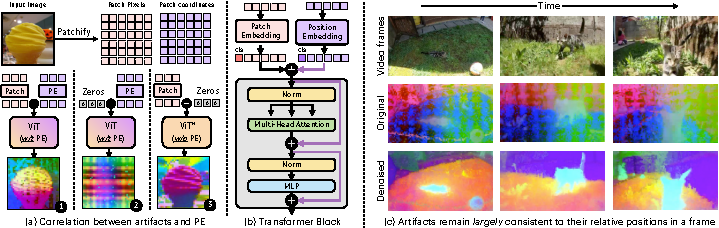
\includegraphics[width=\linewidth]{figures/fig3_pe_illustration.pdf}
    \caption{
        \textbf{Impact of positional embeddings in ViTs.} (a) Comparison between DINOv2 ViTs \cite{oquab2023dinov2} trained with and without positional embeddings ((``ViT'' v.s. ``ViT$^*$''). We show feature maps from (1) a standard ViT, (2) a ViT using only positional embeddings (PE) as input, emphasizing the emergence of artifacts, and (3) a PE-free ViT$^*$, displaying a clear absence of these artifacts. In the figure, ``Patch'': patch embedding, ``PE'': position embedding. (b) Illustration of how ViT retains and propagates the positional embeddings. (c) Despite significant differences in the context of various frames, the artifacts largely maintain a consistent relative position in the images (central row). Our \ours effectively denoises these artifacts, demonstrated in the final row.
    }
    \label{fig:vit_arch}
\end{figure}
%##################################################################################################

